\section{Schema Logico Relazionale}

\begin{itemize}
	\item Esami(\underline{CodiceEsame}, Nome, CFU, link)
	\item AccountTemporanei(\underline{Matricola}, Nome,
	      Cognome, CorsoDiStudio*, Email, Stato)
	\item EsamiSostenuti(\underline{Studente*},
	      \underline{Esame*}, Voto)
	\item CorsiDiStudio(\underline{CodiceCorso}, Nome,
	      Università, Dipartimento,CFUObbligatori,
	      CFUComplementari, CFULiberaScelta)
	\item EsamiECorsi(\underline{Esame*}, \underline{Corso*},
	      Tipologia)
	\item AccountAmministrativi(\underline{CodiceProfessore},
	      Nome, Cognome, Email)
	\item Delibere(\underline{CodiceDelibera}, DataRichiesta,
	      StudenteRichiedente*, Tipologia)
	\item Responsabili(\underline{Professore*},
	      \underline{Delibera*})
	\item EsamiConvalidati(\underline{Delibera*},
	      \underline{Esame*}, Voto)
	\item RiconoscimentoCrediti(\underline{CodiceDelibera*},
	      NomeAttività, CFU)
	\item Ricongiungimenti(\underline{CodiceDelibera*},
	      AnnoInterruzione, AnnoIscrizione)
	\item AbbreviazioniCarriera(\underline{CodiceDelibera*},
	      CorsoProvenienza*)
	\item Trasferimenti(\underline{CodiceDelibera*},
	      CorsoProvenienza*)
\end{itemize}

\begin{figure}[H]
	\centering
	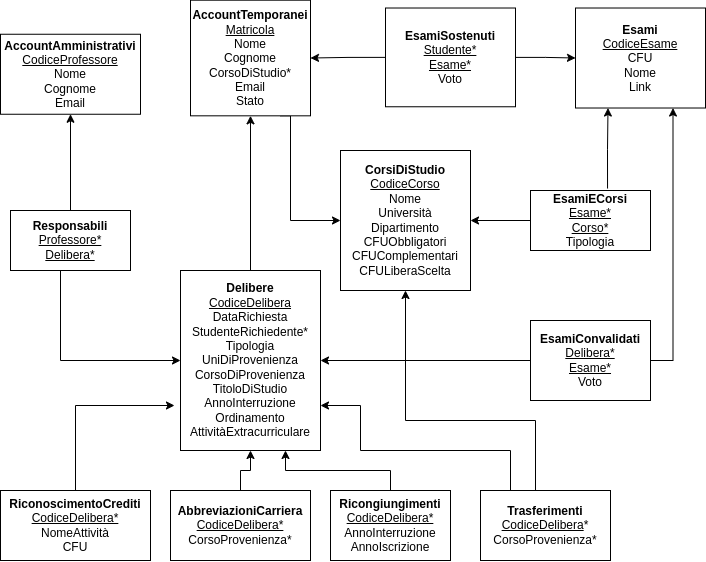
\includegraphics[width=\textwidth]{relazionale.png}
	\caption{Schema logico relazionale}
	\label{Schema logico relazionale}
\end{figure}

Lo schema soddisfa la forma normale di Boyce-Codd perchè in
tutte le dipendenze funzionali della forma \(X \rightarrow Y\),
X è superchiave.

